\documentclass{article}

\title{	
	\normalfont\normalsize 
	\rule{\linewidth}{0.5pt}\\ % Thin top horizontal rule
	\vspace{14pt} % Whitespace
	{\LARGE MATH401 Assignment 4 \\ % The assignment title
    \large \textit{} \\}
	\vspace{6pt} % Whitespace
	\rule{\linewidth}{1pt}\\ % Thick bottom horizontal rule
}

\author{Elliott Hughes}
\date{\normalsize\today}
\usepackage{tikz}
\usetikzlibrary{arrows,automata}
\usetikzlibrary{positioning}
\usetikzlibrary{arrows.meta,positioning}
\usepackage{mdframed}
\usepackage{amsmath}
\usepackage{amssymb}
\usepackage{graphicx}
\graphicspath{ {./Images/Assignment_4/} }
\usepackage{commath}
\usepackage{textcomp}
\usepackage{gensymb}
\usepackage{float}
\usepackage{hyperref}
\usepackage[margin=1in]{geometry}
\usepackage{caption}
\usepackage{subcaption}
\usepackage{sectsty}
\usepackage{titlesec}
\usepackage[title]{appendix}


\begin{document}

\maketitle

\subsection*{Q77}
Let $X$ be a metric space, $T:X \rightarrow X$ a continuous function, $\Omega$ an attracting set 
and $B(\Omega)$ the corresponding basin of attraction. Note furthermore that by definition there 
must exist $U$ an open set such that $\Omega \subset U \subseteq B(\Omega)$. 
Suppose $x \in B(\Omega)$. Since the $\omega$-limit set of $x$ is a subset of $\Omega$ it follows that 
there exists a subsequence $\{n_1,n_2,\dots\}$ such 
that $T^{n_k}(x)$ approaches a point $x^*$ in $\Omega$. Thus for some $N \in \mathbb{N}$, $T^N(x) \in U$ 
as $U$ is open and $\Omega \subset U$ (the subsequence must enter every open neighborhood of 
$x^*$). Therefore $x \in T^{-N}(U)$ and since $T$ preserves continuity it follows that $T^{-N}(U)$ 
is open. Furthermore for every point $y \in T^{-N}(U)$ we have that

\begin{equation}\label{eq:forward_orbits_have_same_omega_set}
	\omega(y) = \lim_{n \rightarrow \infty} \cap_{k =n}^\infty \overline{\mathcal{O}(T^k(y))} = \omega(T^N(y)) \subset \Omega
\end{equation}

Therefore every point in $B(\Omega)$ is contained in an open set in $B(\Omega)$ and so $B(\Omega)$ is 
open. 

\paragraph{}
It remains to consider the behavior of the boundary $\partial B(\Omega) = \overline{B(\Omega)}\backslash B(\Omega)$. 
Since $\Omega$ is attracting it follows that $T(B(\Omega)) \subseteq B(\Omega)$ (as points outside 
this basin do not have $\omega$-limit sets that are in $\Omega$ and by \autoref{eq:forward_orbits_have_same_omega_set} 
this is a contradiction). Therefore $\overline{T(B(\Omega))} \subseteq \overline{B(\Omega)}$ 
and by the continuity of $T$ it follows that $T(\overline{B(\Omega)}) \subseteq \overline{B(\Omega)}$. It is then 
useful to rewrite this as 

\begin{equation*}
	T(\overline{B(\Omega)}) = T(B(\Omega) \cup \partial B(\Omega)) \subseteq B(\Omega) \cup \partial B(\Omega)
\end{equation*}

If $x \in \partial B(\Omega)$ but $T(x) \in B(\Omega)$ this would imply that $x \in B(\Omega)$ by \ref{eq:forward_orbits_have_same_omega_set}. 
However since $B(\Omega)$ is open and since for every open set $N$ containing $x \in \partial B(\Omega)$, $N$ also contains 
points not in $B(\Omega)$ this is a contradiction. Therefore $T(\partial B(\Omega)) \subset X\backslash B(\Omega)$. Consequently 
by the equation above it follows that $T(\partial B(\Omega)) \subseteq \partial B(\Omega)$ and the 
boundary is an invariant set.

\subsection*{Q94}
Consider the orbit of $x = 1/2$ under this tent map. The forward orbit is the set $\{1/2,1/\sqrt{2},1-1/\sqrt{2},\sqrt{2}-1,2-\sqrt{2}\}$ 
as $2 - \sqrt{2}$ is fixed under the action of $T$. This suggests a natural covering of the 
interval $[0,1]$ with the following closed sets:

\begin{align*}
	I_0 &= [0,\sqrt{2}-1] \\
	I_1 &= [\sqrt{2}-1,1/2] \\
	I_2 &= [1/2,2-\sqrt{2}] \\
	I_3 &= [2-\sqrt{2},1/\sqrt{2}] \\
	I_4 &= [1/\sqrt{2},1]
\end{align*}

Consider the images of these subsets under $T$. In particular 

\begin{align*}
	I_0 \cup I_1 \cup I_2 &\subset T(I_0) \\
	I_3 &\subset T(I_1) \\
	I_3 &\subset T(I_2) \\
	I_1 \cup I_2 &\subset T(I_3) \\
	I_0 &\subset T(I_4)
\end{align*}

We can express this system of coverings as a graph (\autoref{fig:dir_graph})

\begin{figure}[H]
	\centering
	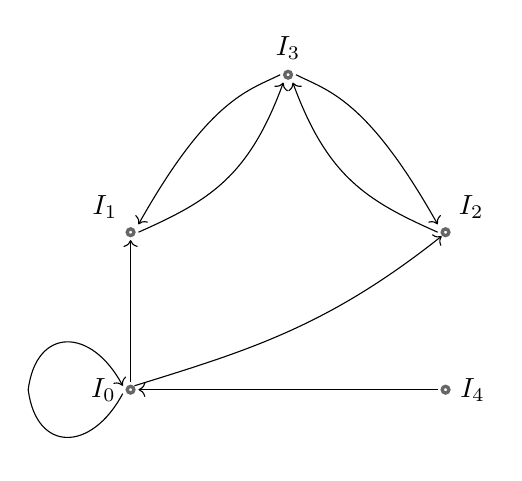
\begin{tikzpicture}[point/.style={circle, very thick, draw=black!60,inner sep = 0.3mm}]
		\node[point,label=left:{$I_0$}] at (-2,0) {};
		\node[point,label=right:{$I_4$}] at (2,0) {};
		\node[point,label=above left:{$I_1$}] at (-2,2) {};
		\node[point,label=above right:{$I_2$}] at (2,2) {};
		\node[point,label=above:{$I_3$}] at (0,4) {}; 
		
		\draw[->] (1.9,0) -> (-1.9,0);
		\draw[->] (-2.1,-0.05) .. controls (-2.5,-0.8) and (-3.2,-0.8) .. (-3.3,0) ..
			controls (-3.2,0.8) and (-2.5,0.8) .. (-2.1,0.05);
		\draw[->] (-2,0.1) -> (-2,1.9);
		\draw[->] (-1.95,0.05) .. controls (-0.5,0.5) and (0.5,0.8) .. (1.95,1.95);
		\draw[->] (-1.9,2) .. controls (-1,2.4) and (-0.5,2.7) .. (-0.06,3.9);
		\draw[<-] (-1.9,2.1) .. controls (-1,3.7) and (-0.5,3.8) .. (-0.1,4);
		\draw[->] (1.9,2) .. controls (1,2.4) and (0.5,2.7) .. (0.06,3.9);
		\draw[<-] (1.9,2.1) .. controls (1,3.7) and (0.5,3.8) .. (0.1,4);

	\end{tikzpicture}
	\caption{A directed graph of the coverings of the intervals.}
	\label{fig:dir_graph}
\end{figure}

\paragraph{}
This graph is sufficient to show that the set of excluded cylinders in the coding proposed 
in the question statement is not a sub-shift of finite type. Consider a cylinder of the form 
1101...1 where 1...1 is a cylinder of even length formed entirely of 1s. From the 
graph above an orbit in this cylinder must be in the cylinder $I_2I_3I_1I_3...I_2$ under the coding 
induced by the graph. However a point in $I_2$ cannot transition to the left-hand side of the interval, 
so the cylinder $1101...10$ is excluded for any finite cylinder 1...1 of even length.

\paragraph{}
This generates an infinite set of excluded cylinders. It remains to show that we cannot construct 
a shorter excluded cylinder that enables us to write the set of excluded cylinders as some smaller finite 
set. Such a cylinder would have to be of the form 1...10 for some finite length of 1s. It is 
clear that one can construct a cylinder $...I_3I_0$ (under the coding induced by the graph) where each of the preceding terms in the 
cylinder are either $I_2$ or $I_3$. Since each component interval contains points other than $1/2$ and 
this cylinder is not excluded under the coding induced by the graph, this implies an orbit (other than that of $1/2$) 
must exist and will lie in the cylinder 1...10 in question. Therefore we cannot construct a smaller 
cylinder that would reduce the set of excluded cylinders to a finite set and so the coding 
induced in the question is not a sub-shift of finite type.

\subsection*{Q95}
Since there are relatively few matrices which fit the criteria to be transition matrices $A \in \{0,1\}^{2 \times 2}$, 
it is straightforward to enumerate all of them.

\begin{equation*}
	\begin{split}
	A_0 = \begin{bmatrix}0 & 0 \\ 0 & 0\end{bmatrix} \qquad A_1 = \begin{bmatrix}1 & 0 \\ 0 & 0\end{bmatrix} \qquad A_2 = \begin{bmatrix}0 & 1 \\ 0 & 0\end{bmatrix} \\
	A_3 = \begin{bmatrix}0 & 0 \\ 1 & 0\end{bmatrix} \qquad A_4 = \begin{bmatrix}0 & 0 \\ 0 & 1\end{bmatrix} \qquad A_5 = \begin{bmatrix}1 & 1 \\ 0 & 0\end{bmatrix} \\
	A_6 = \begin{bmatrix}1 & 0 \\ 1 & 0\end{bmatrix} \qquad A_7 = \begin{bmatrix}0 & 0 \\ 1 & 1\end{bmatrix} \qquad A_8 = \begin{bmatrix}0 & 1 \\ 0 & 1\end{bmatrix} \\
	A_9 = \begin{bmatrix}1 & 0 \\ 0 & 1\end{bmatrix} \qquad A_{10} = \begin{bmatrix}0 & 1 \\ 1 & 0\end{bmatrix} \qquad A_{11} = \begin{bmatrix}1 & 0 \\ 1 & 1\end{bmatrix} \hspace{-4pt}\\
	A_{12} = \begin{bmatrix}0 & 1 \\ 1 & 1\end{bmatrix} \qquad A_{13} = \begin{bmatrix}1 & 1 \\ 1 & 0\end{bmatrix} \qquad A_{14} = \begin{bmatrix}1 & 1 \\ 0 & 1\end{bmatrix} \hspace{-4pt}\\
	A_{15} = \begin{bmatrix}1 & 1\\ 1 & 1\end{bmatrix} \hspace{77pt}
	\end{split}
\end{equation*}

It is now straightforward to discern which of the matrices correspond to which of the categories 
of interest.

\paragraph{(a)}
Clearly the spaces induced by $A_0$, $A_2$ and $A_3$ do not contain any infinite strings, so these string spaces are 
empty. The spaces induced by $A_1$, $A_4$, $A_5$, $A_7$ and $A_{10}$ contain only one infinite string so these spaces are also finite. 
Meanwhile, there are two infinite strings in the $A_6$, $A_8$ and $A_9$. The graphs that correspond 
to the matrices $A_{11}$ and $A_{14}$ are isomorphic to the following graph 

\begin{figure}[H]
	\centering
	\begin{tikzpicture}[point/.style={circle, very thick, draw=black!60,inner sep = 0.3mm}]
		\node[point] at (-2,0) {};
		\node[point] at (2,0) {};
		
		\draw[->] (1.9,0) -> (-1.9,0);
		\draw[->] (-2.1,-0.05) .. controls (-2.5,-0.8) and (-3.2,-0.8) .. (-3.3,0) ..
			controls (-3.2,0.8) and (-2.5,0.8) .. (-2.1,0.05);
		\draw[->] (2.1,-0.05) .. controls (2.5,-0.8) and (3.2,-0.8) .. (3.3,0) ..
			controls (3.2,0.8) and (2.5,0.8) .. (2.1,0.05);
	\end{tikzpicture}
\end{figure}

Clearly there are infinitely many strings of the form 1000..., 1100..., 1110... or 0111..., 0011... or 
0001.... depending on the particular matrix, so these spaces are not infinite. Then $A_{12}$ and $A_{13}$ have 
graphs that are isomorphic to following graph

\begin{figure}[H]
	\centering
	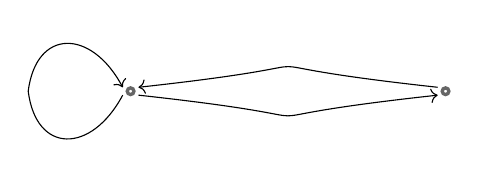
\begin{tikzpicture}[point/.style={circle, very thick, draw=black!60,inner sep = 0.3mm}]
		\node[point] at (-2,0) {};
		\node[point] at (2,0) {};
		
		\draw[->] (1.9,0.05) .. controls (-1.3,0.4) and (1.3,0.4) .. (-1.9,0.05);
		\draw[<-] (1.9,-0.05) .. controls (-1.3,-0.4) and (1.3,-0.4) .. (-1.9,-0.05);
		\draw[->] (-2.1,-0.05) .. controls (-2.5,-0.8) and (-3.2,-0.8) .. (-3.3,0) ..
		controls (-3.2,0.8) and (-2.5,0.8) .. (-2.1,0.05);
	\end{tikzpicture}
\end{figure}

Clearly there are infinitely many strings of the form 1000..., 0100..., 0010,... or 0111..., 1011..., 
1101... depending on the particular matrix in question. So these matrices induce symbol 
spaces which are infinite. It is hopefully obvious that this implies that $A_{15}$ also induces 
an infinite symbol space. Therefore the transition matrices which induce a finite or empty 
string space are $A_0$, $A_1$, $A_2$, $A_3$, $A_5$, $A_6$, $A_7$, $A_8$, $A_9$ and $A_{10}$.

\paragraph{(b)}
Restricting our analysis to non-empty symbol spaces, if we require periodic points under the left-shift 
$\sigma$ to be dense then we must be able to construct strings which are periodic and arbitrarily 
close to any other string in this space. Spaces which only contain one periodic sequence (and no other sequence) obviously 
have dense periodic sequences in $\sigma$. Therefore $A_1$, $A_4$, $A_5$, $A_7$ and $A_{10}$ fulfill this requirement. 
In addition $A_9$ also has dense periodic sequences as it only contains periodic sequences 0000... and 
1111.... Each of $A_6$ and $A_8$ do not contain dense periodic sequences as these have only one 
periodic sequence (either 0000... or 1111...) but also contain a sequence 0111... or 1000... 
which is not arbitrarily close to the periodic sequence.

\paragraph{}
In $A_{11}$ or $A_{14}$ there are two periodic points in both of these string spaces; 0000... and 1111.... However each 
of these spaces contain either the string 0111... or 1000... which is not arbitrarily close to 
either of the periodic points in these string spaces. In the case of $A_{12}$ or $A_{13}$ for a cylinder of length $n$ in this space, one can choose a string which repeats this 
cylinder infinitely, potentially with a finite amount of `padding' to connect the end of 
one cylinder to the start of the next. Therefore periodic points are dense in $A_{12}$ and $A_{13}$. 
By a similar argument it should be clear that $A_{15}$ also has dense periodic points. Therefore 
the set of adjacency matrices which induce spaces with dense periodic orbits under the left shift 
$\sigma$ is $A_1$, $A_4$, $A_5$, $A_7$, $A_9$, $A_{10}$, $A_{12}$, $A_{13}$ and $A_{15}$.

\paragraph{(c)}
A shift space has a dense orbit if for every sequence of length $n$ in this shift space, there exists 
some orbit which includes this sequence. Clearly spaces which only contain one string will fulfill this requirement (e.g. $A_1$, $A_4$, $A_5$, $A_7$ and $A_{10}$). Furthermore 
since every cylinder in the space induced by $A_6$ is either 1000...0 or 0000...0 so the orbit of the infinite sequence 1000... is dense in the induced space. By an identical argument, 
$A_8$ also fulfills this requirement. 

\paragraph{}
However the space induced by $A_9$ does not have dense orbits as it is impossible to transition 
between the two periodic points 0000... and 1111.... $A_{11}$ also does not induce a shift space which contains a dense orbit as an 
infinite sequence in this space is either a infinite string containing only 1s or the 
first $n$ digits are 1 for some $n \in \mathbb{N}$ and the rest are zeros. Therefore for 
any particular infinite sequence there exists some cylinder with a finite number of leading 1s (e.g. one more than the 
number of leading ones in the infinite sequence in question) followed by some finite number of 
zeros which is not excluded and does not appear in the infinite sequence. An identical argument also suffices 
to eliminate $A_{14}$. 

\paragraph{}
However there is a dense orbit in the shift spaces induced by $A_{12}$ and $A_{13}$. In both 
cases the transitivity of the graph means that a dense orbit can be constructed by choosing some initial point 
and then appending each cylinder of interest to the end of the finite sequence (potentially with 
a finite amount of padding to connect the end of one cylinder to the start of the next). The 
preceding argument also applies to $A_{15}$, so the final set of adjacency matrices which induce 
shift spaces with a dense orbit are $A_1$, $A_4$, $A_5$, $A_7$, $A_8$, $A_{10}$, $A_{12}$, $A_{13}$ 
and $A_{15}$.

\subsection*{Q100}
Histograms were computed using the Numpy python package, with plotting routines from Matplotlib. 
Code for this question and Q107 is available in appendix A. As one would expect, rotations by 
a rational angle produce orbits which are concentrated in a finite set of small sub-intervals, 
while rotations by an irrational angle lead to orbits which are dense in the interval and 
approach a pseudo-uniform distribution in the limit.

\subsection*{Rotation by $\omega = 2/3$}

\begin{figure}[H]
	\centering
	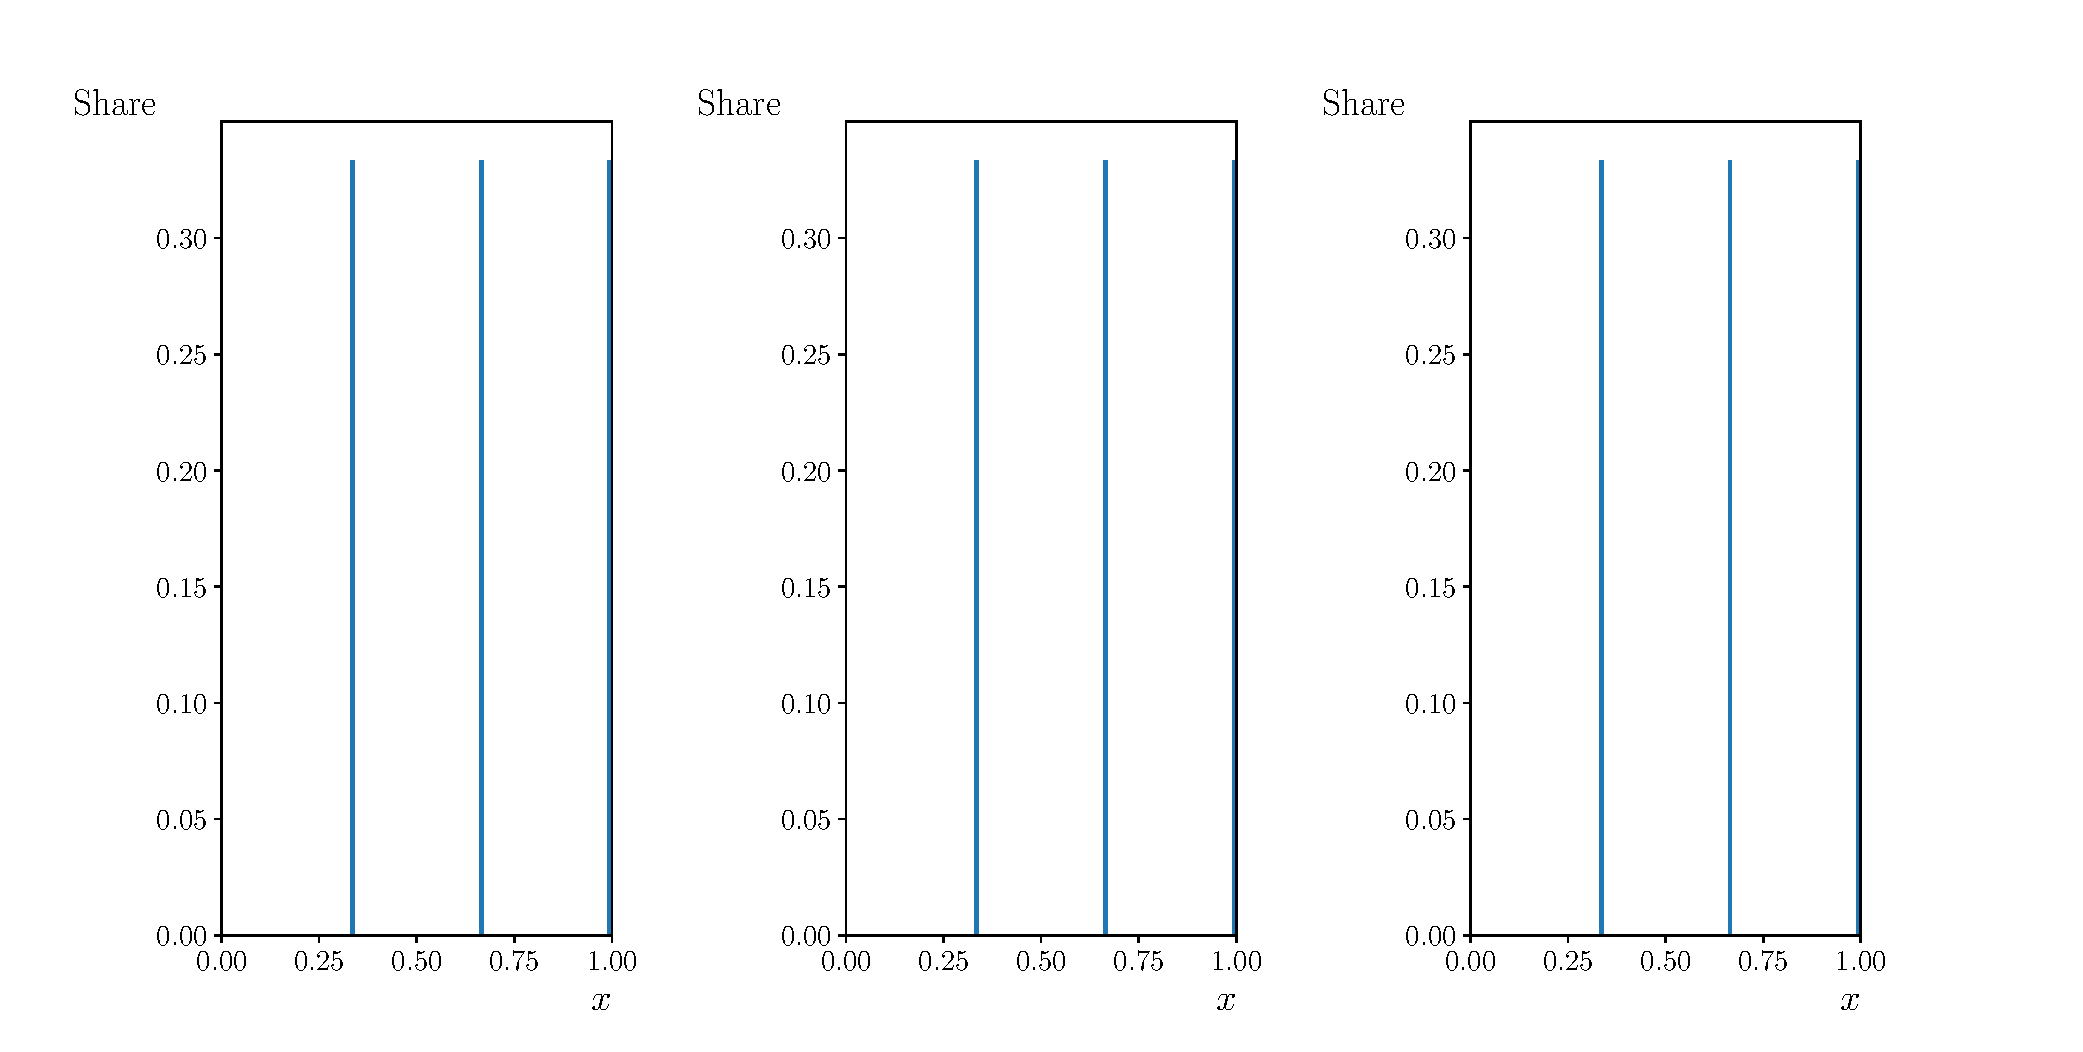
\includegraphics[scale = 0.55]{Q100_Hist_Rot_23.eps}
	\caption{A Histogram of the first $10^n$ (from left to right $n = 4,5,6$) orbits of $x_0 = 0$ under the map $T(x) = x + \omega$. 
	Counts are normalized so each bin gives the share of orbits landing in that particular sub-interval.}
\end{figure}

\subsection*{Rotation by $\omega = 21/34$}

\begin{figure}[H]
	\centering
	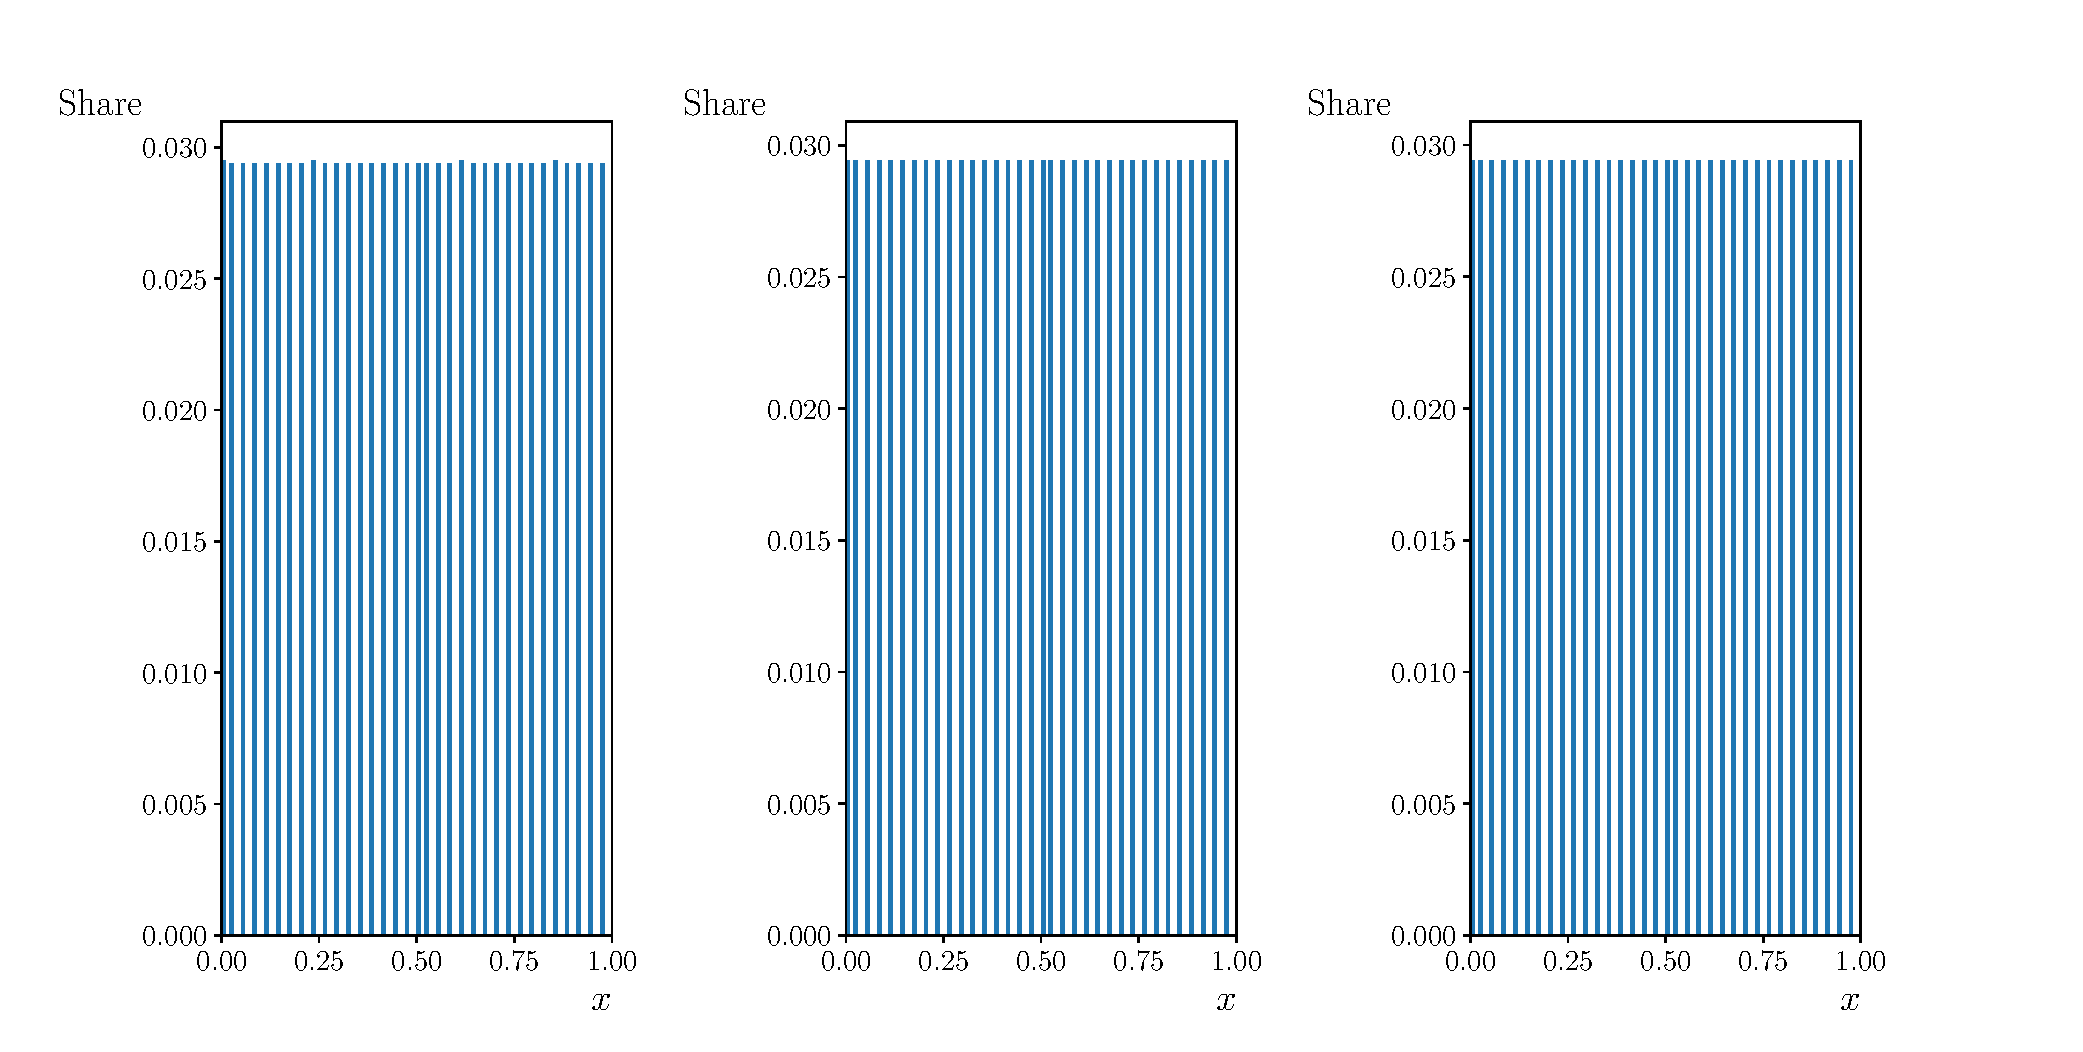
\includegraphics[scale = 0.55]{Q100_Hist_Rot_34.eps}
	\caption{A Histogram of the first $10^n$ (from left to right $n = 4,5,6$) orbits of $x_0 = 0$ under the map $T(x) = x + \omega$. 
	Counts are normalized so each bin gives the share of orbits landing in that particular sub-interval.}
\end{figure}

\subsection*{Rotation by $\omega = (\sqrt{5} -1)/2$}

\begin{figure}[H]
	\centering
	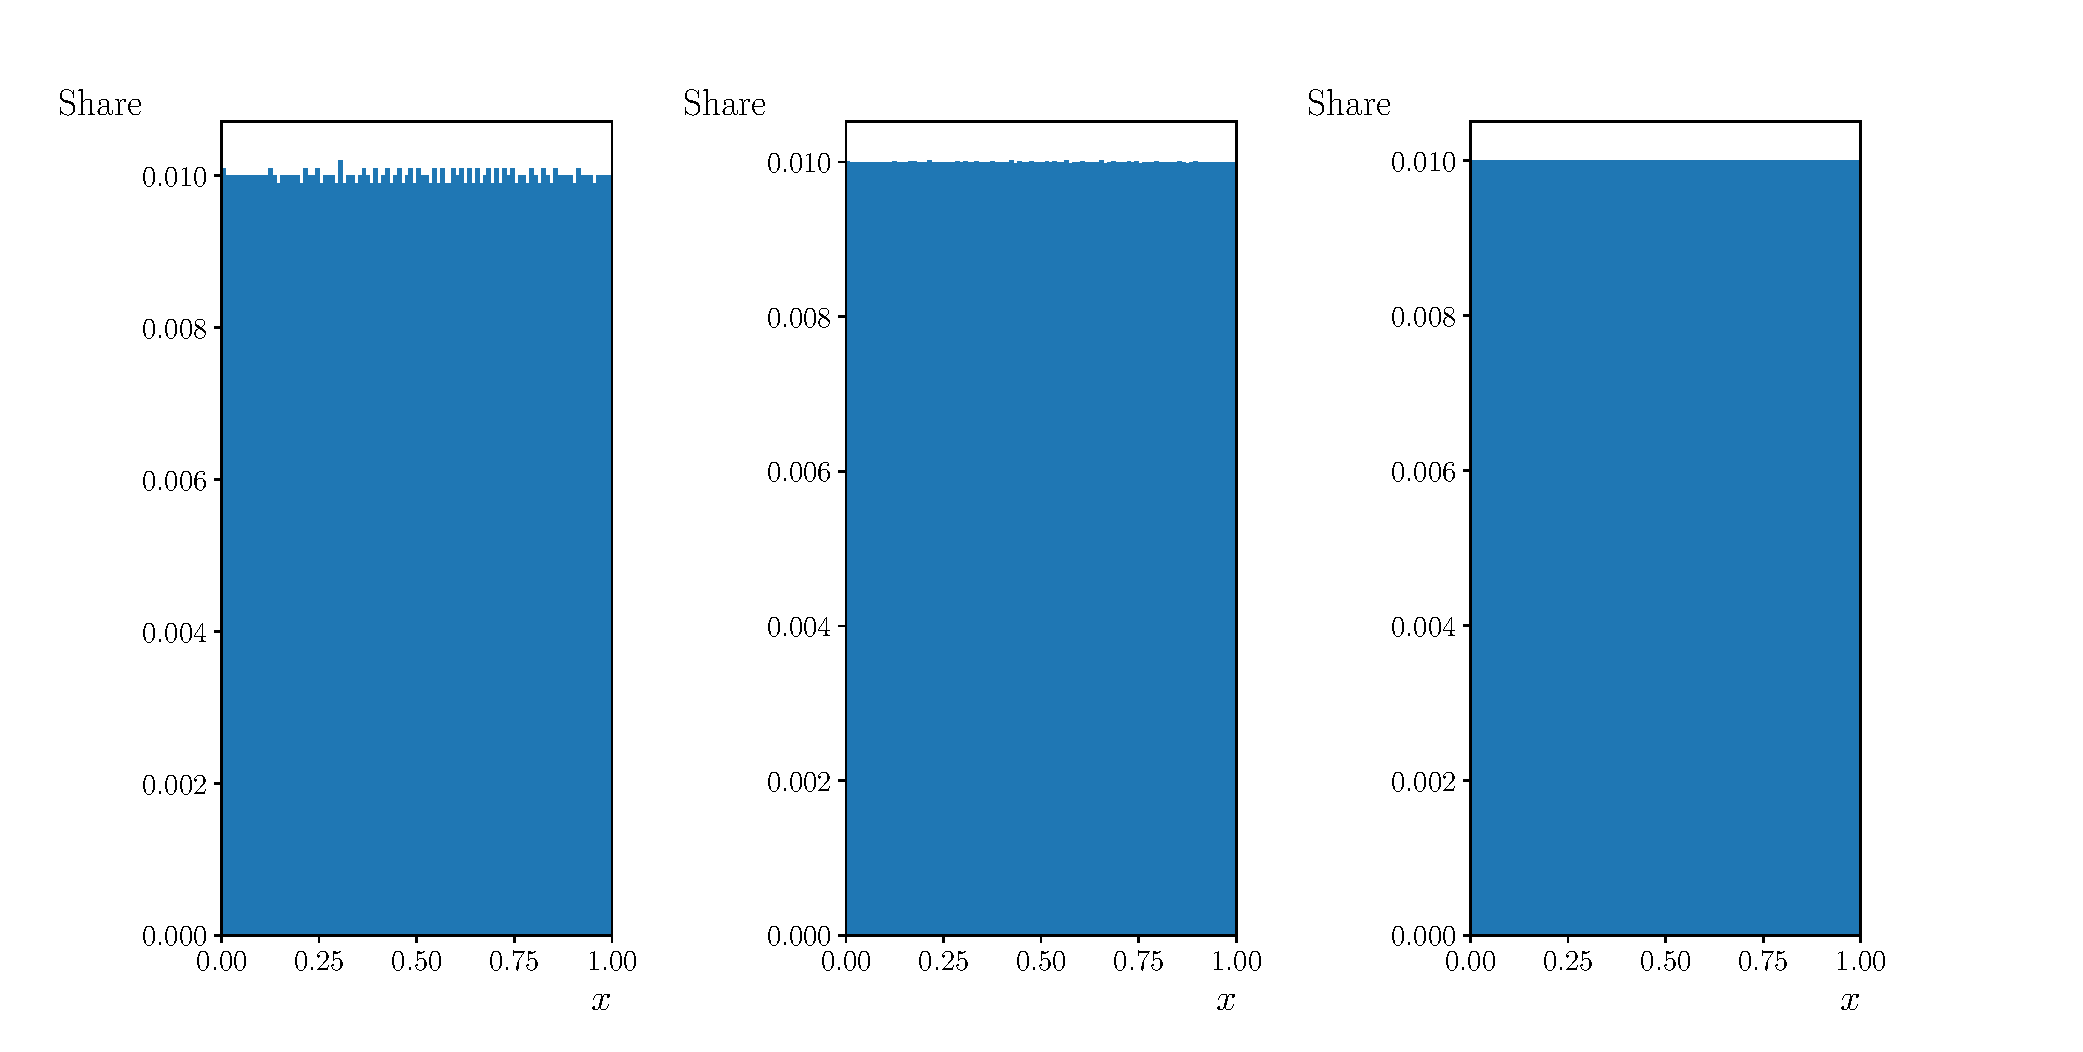
\includegraphics[scale = 0.55]{Q100_Hist_Rot_root5.eps}
	\caption{A Histogram of the first $10^n$ (from left to right $n = 4,5,6$) orbits of $x_0 = 0$ under the map $T(x) = x + \omega$. 
	Counts are normalized so each bin gives the share of orbits landing in that particular sub-interval.}
\end{figure}

\subsection*{Rotation by $\omega = 1/\sqrt{3}$}

\begin{figure}[H]
	\centering
	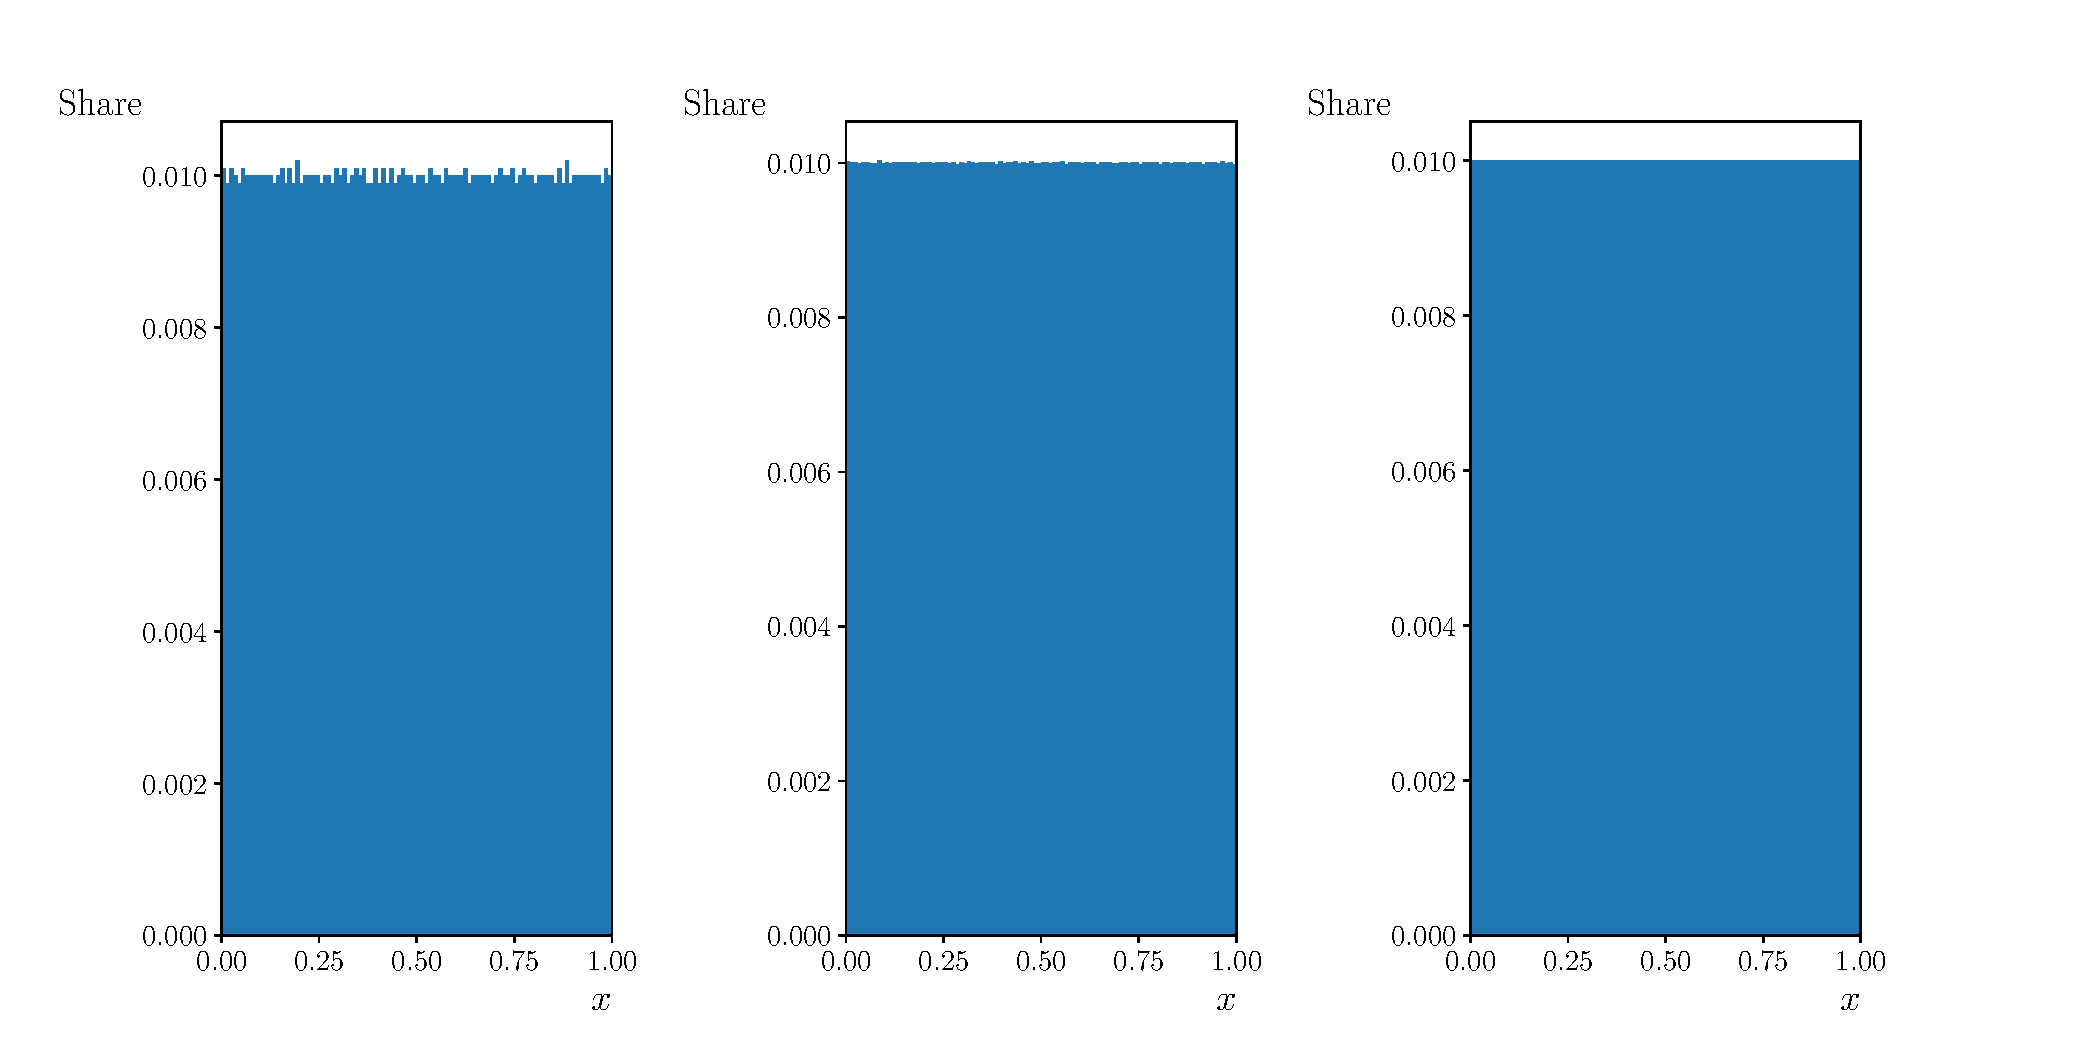
\includegraphics[scale = 0.55]{Q100_Hist_Rot_root3.eps}
	\caption{A Histogram of the first $10^n$ (from left to right $n = 4,5,6$) orbits of $x_0 = 0$ under the map $T(x) = x + \omega$. 
	Counts are normalized so each bin gives the share of orbits landing in that particular sub-interval.}
\end{figure}

\subsection*{Q107}
\paragraph{Q100}
It is straightforward to approximate the action of this system on $[0,1)$ with an Ulam matrix. One 
interesting point is that the transfer of mass appears similar under rotations by both an 
irrational and a rational angle (at least for a small number of iterations) even though the orbits 
of any particular point are quite different under each action.

\begin{figure}[H]
	\centering
	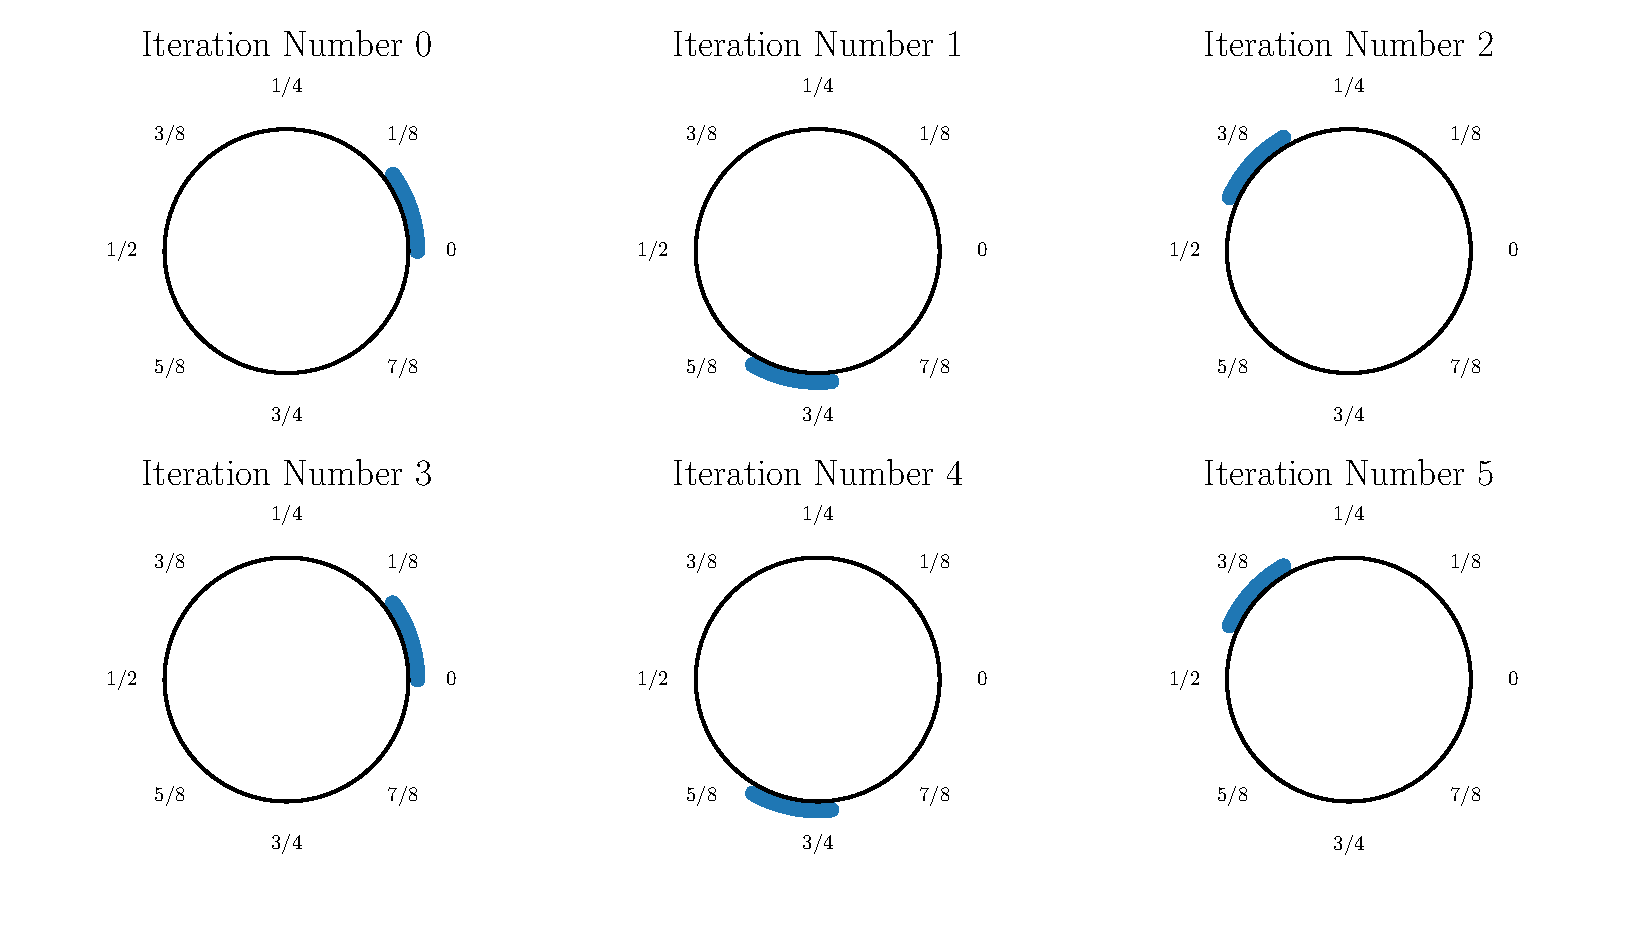
\includegraphics[scale = 0.6]{Q107_Ulam_Rot_23.eps}
	\caption{The first five rotations by a rational angle ($2/3$) of a mass distributed uniformly from 0 to 0.1. Angles 
	have been scaled so that a rotation of $2/3$ is equivalent to a rotation by $4\pi/3$ radians.}
\end{figure}

\begin{figure}[H]
	\centering
	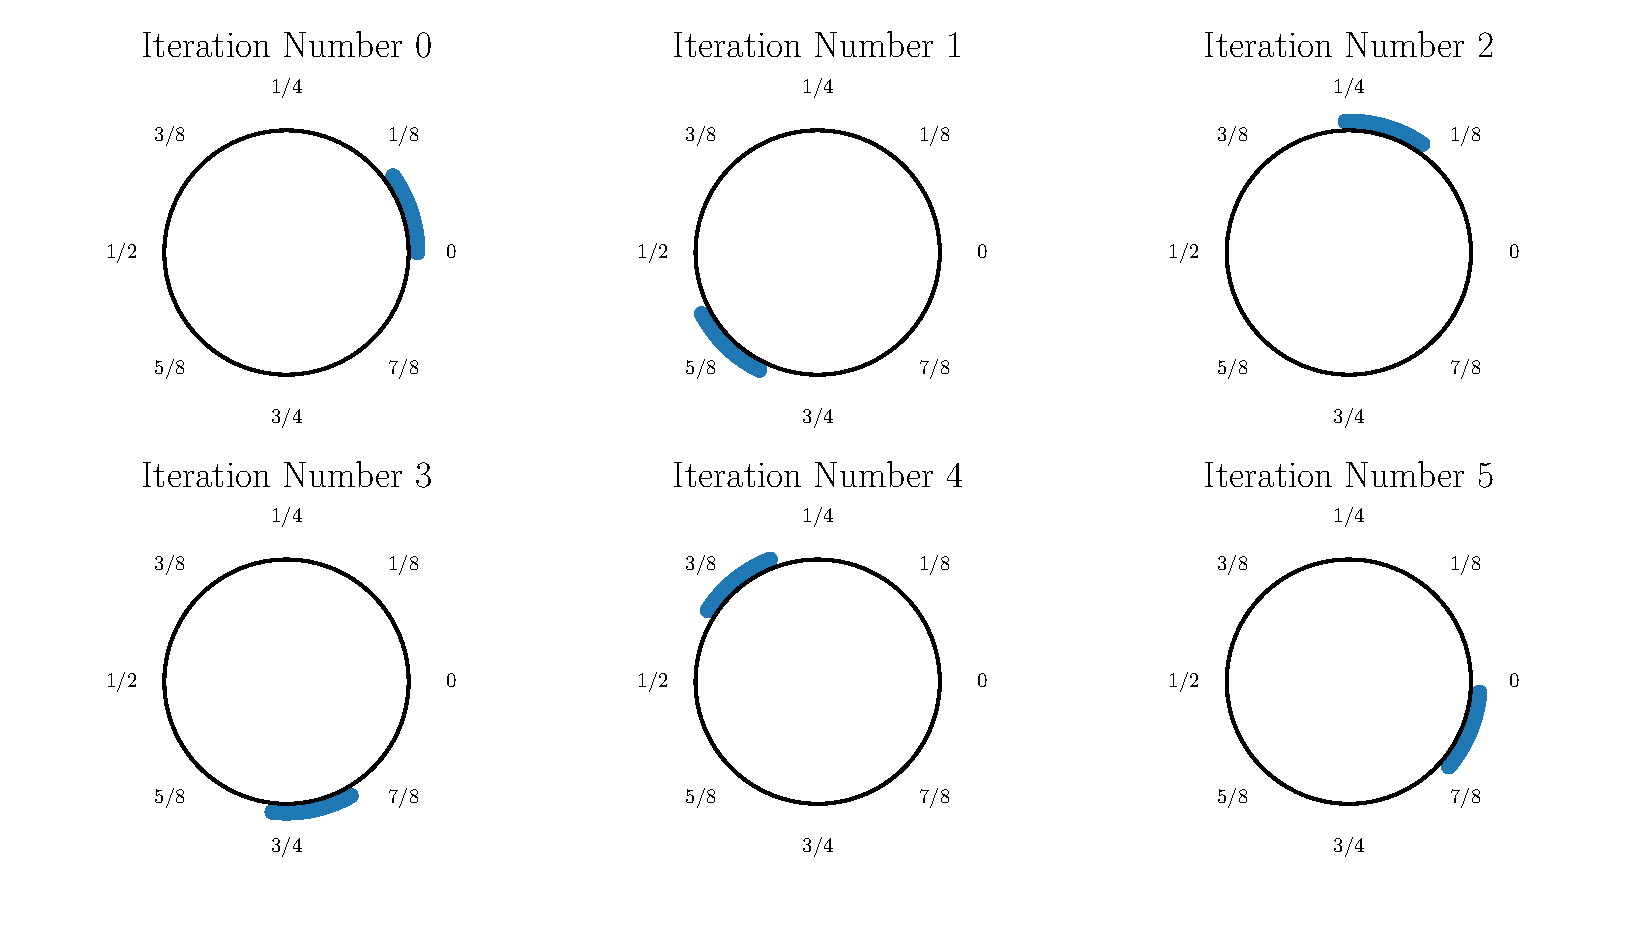
\includegraphics[scale = 0.6]{Q107_Ulam_Rot_root3.eps}
	\caption{The first five rotations by a irrational angle ($1/\sqrt{3}$) of a mass distributed uniformly from 0 to 0.1. Angles 
	have been scaled so that a rotation of $1/\sqrt{3}$ is equivalent to a rotation by $2\pi/\sqrt{3}$ radians.}
\end{figure}

Rotation plots for the remaining two angles are in appendix B.

\paragraph{Q102}
While this map is defined on an infinite domain, we will restrict our attention to the region where 
the initial distribution of mass is non-zero (e.g. $[0,2]$). It is easy to see that on this 
interval all mass will be drawn towards the center-point under repeated iterations of $T$.

\begin{figure}[H]
	\centering
	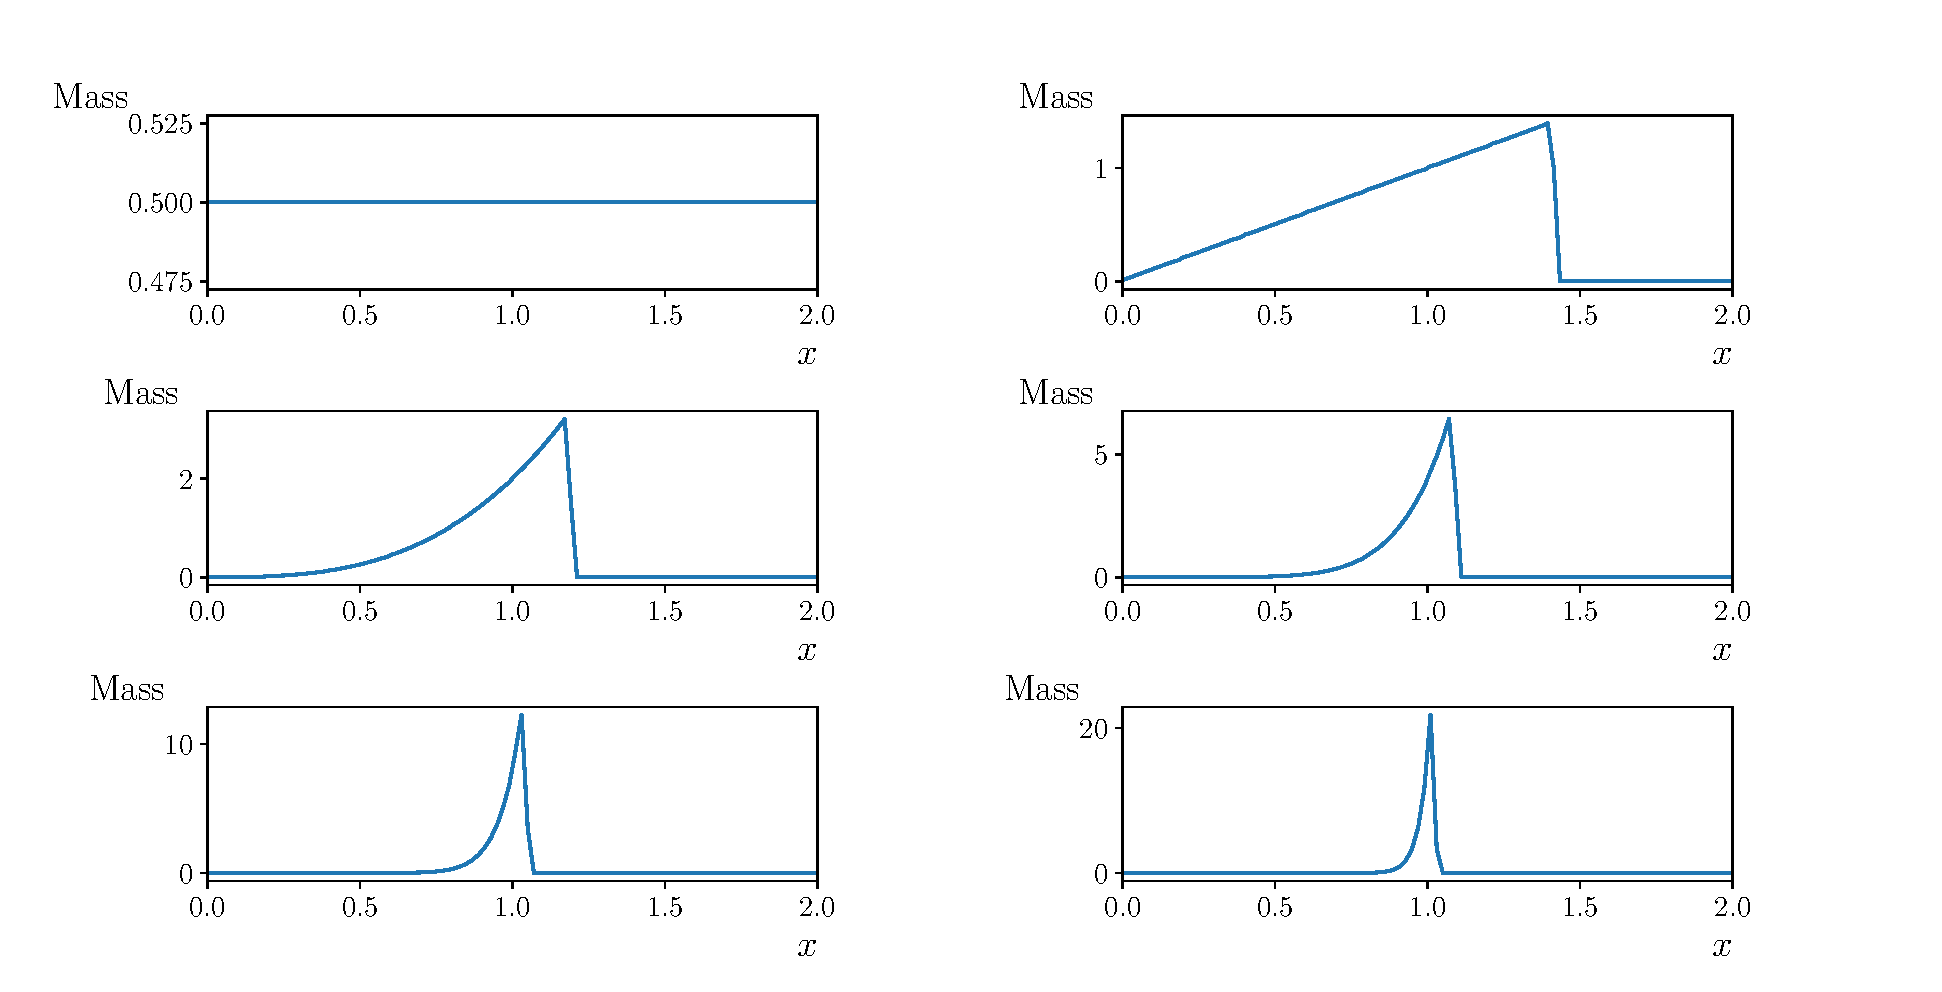
\includegraphics[scale = 0.55]{Q107_102_Mass_Trans.eps}
	\caption{Transit of a mass of height 0.5 for $0 < x < 2$ under five iterations of $T$. Note 
	the concentration of the mass around the center point.}
\end{figure}

Indeed, the largest eigenvalue of the Ulam matrix (when normalized) corresponds to a eigenvector 
which is 1 at $x = 1$ and zero elsewhere. 
Therefore, in the limit we would expect initial distributions $f(x)$ to tend towards the 
Dirac delta distribution under repeated applications of $\mathcal{P}$.

\begin{figure}[H]
	\centering
	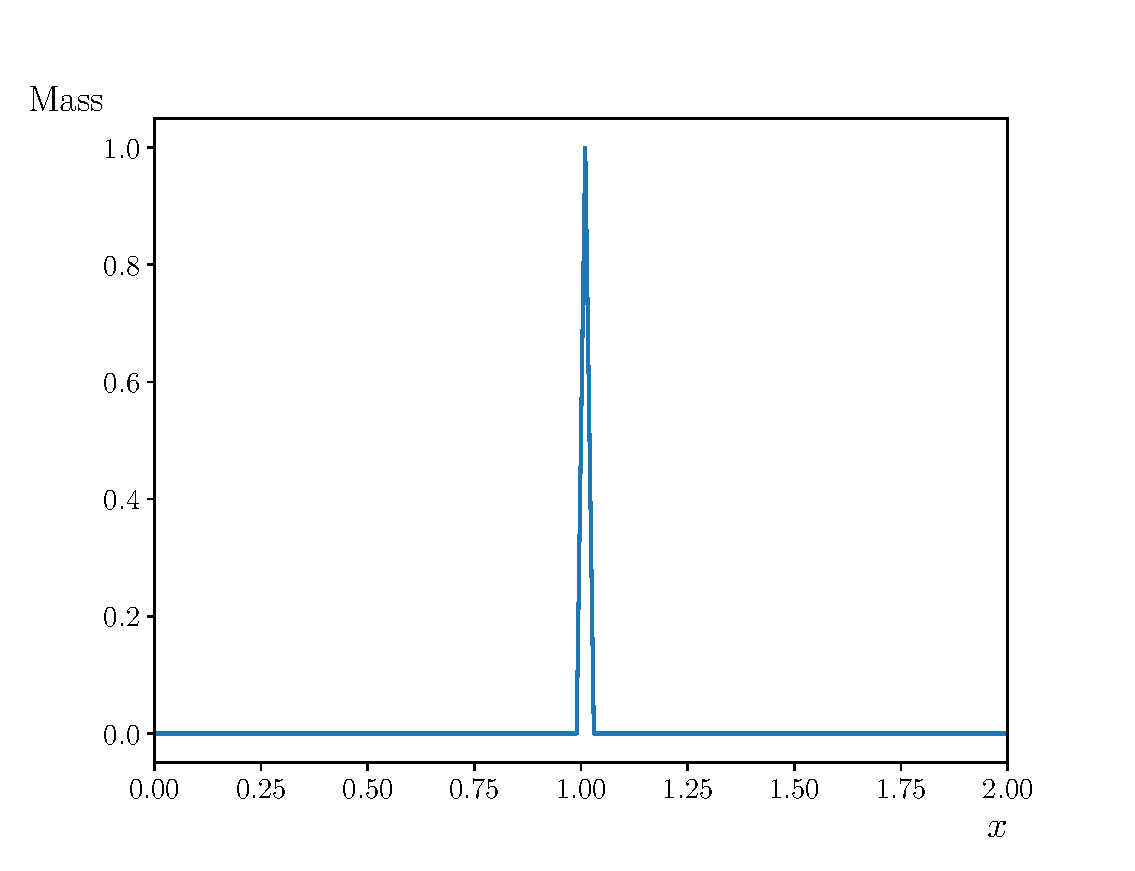
\includegraphics[scale = 0.55]{Q107_102_Mass_Ets.eps}
	\caption{The eigenvector corresponding to the largest eigenvalue (e.g. the limiting distribution) of $T$ normalized so that the height of 
	the peak is 1.}
\end{figure}



\begin{appendices}
\section*{Appendix A -- Code for Q100 and Q107}
\subsection*{Q100}
\begin{verbatim}
# plot parameters etc
import numpy as np
import matplotlib.pyplot as plt
plt.rcParams.update({
    "text.usetex": True,
    "font.family": "serif",
    "font.serif": ["Computer Modern Roman"]})

# histogram generator
def hist_gen(x0,shift,length):
    # create the map
    def q100_func(x,shift):
        return np.modf(x+shift)[0]
    
    # create the 10^4/5/6 orbits function
    orbits = []
    weights = []
    for k in length:
        # create new orbit 
        orbit = np.empty((10**k,))
        x_new = x0
        for i in range(1,10**k):
            x_new = q100_func(x_new,shift)
            orbit[i] = x_new
        orbits += [orbit]
        weights += [np.ones_like(orbit) / len(orbit)]

    # plot the output ax1
    fig, (ax1, ax2, ax3) = plt.subplots(1,3)
    ax1.hist(orbits[0], bins = 100, range = (0,1), weights = weights[0])
    ax1.set_xlim(0,1)
    ax1.set_xlabel('$x$', loc = 'right', fontsize = 18)
    ax1.set_ylabel('Share', loc = 'top', rotation = 'horizontal', fontsize = 18)
    ax1.yaxis.labelpad = 0
    ax1.tick_params(labelsize = 14)
    # do the same for x2
    ax2.hist(orbits[1], bins = 100, range = (0,1), weights = weights[1])
    ax2.set_xlim(0,1)
    ax2.set_xlabel('$x$', loc = 'right', fontsize = 18)
    ax2.set_ylabel('Share', loc = 'top', rotation = 'horizontal', fontsize = 18)
    ax2.yaxis.labelpad = 0
    ax2.tick_params(labelsize = 14)
    # do x3
    ax3.hist(orbits[2], bins = 100, range = (0,1), weights = weights[2])
    ax3.set_xlim(0,1)
    ax3.set_xlabel('$x$', loc = 'right', fontsize = 18)
    ax3.set_ylabel('Share', loc = 'top', rotation = 'horizontal', fontsize = 18)
    ax3.yaxis.labelpad = 0
    ax3.tick_params(labelsize = 14)

    # tweak padding
    plt.subplots_adjust(left=0.1, bottom=0.1, right=0.9, top=0.9, wspace=0.6, hspace=0.5)

    # return our figure
    return(fig)

# create the required figures and show them
shifts = [2/3,21/34,0.5*(np.sqrt(5)-1),1/np.sqrt(3)]
figs = []
for s in shifts:
    figs += [hist_gen(0,s,(4,5,6))]
plt.show()
\end{verbatim}
\subsection*{Q102}
\begin{verbatim}
	import numpy as np
	from numpy.linalg import eig
	import matplotlib.pyplot as plt
	plt.rcParams.update({
		"text.usetex": True,
		"font.family": "serif",
		"font.serif": ["Computer Modern Roman"]})
	
	# this is the operator for Q100
	def q100_func(x,shift):
		return np.modf(x+shift)[0] 
	
	# this function is the transformed function for Q102 on (0,1]
	def q102_func(x,params):
		return 1/(np.sqrt(1/x -1) + 1)
	
	def ulam_method(func,bins,K,params):
		# take as input a function defined on [0,1] the number of bins and the number of points 
		# inside each bin
	
		# build an array where each row is all the K points in some bin
		x_in_bins = []
		for i in range(bins.shape[0]-1):
			x_in_bins += [np.linspace(bins[i],bins[i+1],K)]
		x_in_bins = np.array(x_in_bins)
	
		# apply the function of interest to the array
		x_trans = func(x_in_bins,params)
	
		# Create the output array 
		Ulam_matrix = np.empty((bins.shape[0]-1,bins.shape[0]-1))
	
		# create each entry in the Ulam matrix
		for j in range(x_in_bins.shape[0]):
			Ulam_matrix[:,j] = np.histogram(x_trans[j,:],bins,density=False)[0]/K
	
		# return the Ulam matrix and the 
		return Ulam_matrix
	
	# draw some pictures for mass transport starting on 0,0.1 for each angle in Q100
	angles = [2/3,21/34,(np.sqrt(5)-1)/2,1/np.sqrt(3)]
	figs = []
	for angle in angles:
		mat_Q100 = ulam_method(q100_func,np.linspace(0,1,1001),100,angle)
		fig, axes = plt.subplots(2,3,subplot_kw={'projection': 'polar'})
		plt.subplots_adjust(left=0.05, bottom=0.1, right=0.95, top=0.9, wspace=0.4, hspace=0.5)
		figs += [fig]
		axes = list(np.reshape(axes,(6,)))
		x_axis = np.linspace(0,1,1000)
		border = 0.85*np.reshape(np.ones((1,1000)),(1000,))
		blob = np.zeros(1000)
		blob[0:100] = 0.1
		counter = 0
		x_reg = x_axis[blob > 0.05]
		axes[0].scatter(2*np.pi*x_reg, np.ones(x_reg.shape[0]))
		axes[0].plot(2*np.pi*x_axis, border,color='black')
		axes[0].set_rticks([])
		axes[0].set_ylim([-1.2,1.2])
		axes[0].set_xticks([])
		axes[0].spines['polar'].set_visible(False)
		axes[0].set_title('Iteration Number ' + str(counter), va = 'bottom', fontsize = 18)
		for ax in axes[1:]:
			counter += 1
			blob= np.matmul(mat_Q100,blob)
			x_reg = x_axis[blob > 0.05]
			ax.scatter(2*np.pi*x_reg, np.ones(x_reg.shape[0]))
			ax.plot(2*np.pi*x_axis, border,color='black')
			ax.set_rticks([])
			ax.set_ylim([-1.2,1.2])
			ax.set_xticks([])
			ax.spines['polar'].set_visible(False)
			ax.set_title('Iteration Number ' + str(counter), va = 'bottom', fontsize = 18)
	
	# get the Ulam matrix for Q102
	max_eigvec = []
	for k in [10,100]:
		mat_Q102 = ulam_method(q102_func,np.linspace(1e-8,1,101),k,0)
		# from this grab the largest eigenvalue and eigenvector
		eigvals_102, eigvec_102 = eig(mat_Q102)
		max_eigval = eigvals_102[np.argmax(np.abs(eigvals_102))]
		max_eigvec += [eigvec_102[:,np.argmax(np.abs(eigvals_102))]]
	
	# use the matrix we have just computed to draw some pictures of mass transport for a blob starting on 0,0.1 
	fig, axes = plt.subplots(3,2)
	plt.subplots_adjust(left=0.1, bottom=0.1, right=0.9, top=0.9, wspace=0.5, hspace=0.7)
	axes = list(np.reshape(axes,6))
	x_axis = np.linspace(0,1,mat_Q102.shape[0])
	blob = np.zeros(mat_Q102.shape[0])
	blob[0:10] = 0.1
	axes[0].plot(x_axis,blob)
	axes[0].set_xlim(0,1)
	axes[0].set_xlabel('$x$', loc = 'right', fontsize = 18)
	axes[0].set_ylabel('Mass', loc = 'top', rotation = 'horizontal', fontsize = 18)
	axes[0].yaxis.labelpad = 0
	axes[0].tick_params(labelsize = 14)
	for ax in axes[1:]:
		blob = np.matmul(mat_Q102,blob)
		ax.plot(x_axis,blob)
		ax.set_xlim(0,1)
		ax.set_xlabel('$x$', loc = 'right', fontsize = 18)
		ax.set_ylabel('Mass', loc = 'top', rotation = 'horizontal', fontsize = 18)
		ax.yaxis.labelpad = 0
		ax.tick_params(labelsize = 14)
	
	# Also plot the eigenvector in a separate figure
	fig2, ax_eig = plt.subplots(1,1)
	ax_eig.plot(np.linspace(0,1,max_eigvec[0].shape[0]),max_eigvec[0]) # plot the eigenvector distribution
	ax_eig.set_xlim(0,1)
	ax_eig.set_xlabel('$x$', loc = 'right', fontsize = 18)
	ax_eig.set_ylabel('Mass', loc = 'top', rotation = 'horizontal', fontsize = 18)
	ax_eig.yaxis.labelpad = 0
	ax_eig.tick_params(labelsize = 14)
	plt.show()
\end{verbatim}

\section*{B -- Rotations by the $\omega = 21/34,\frac{1-\sqrt{5}}{2}$}

\begin{figure}[H]
	\centering
	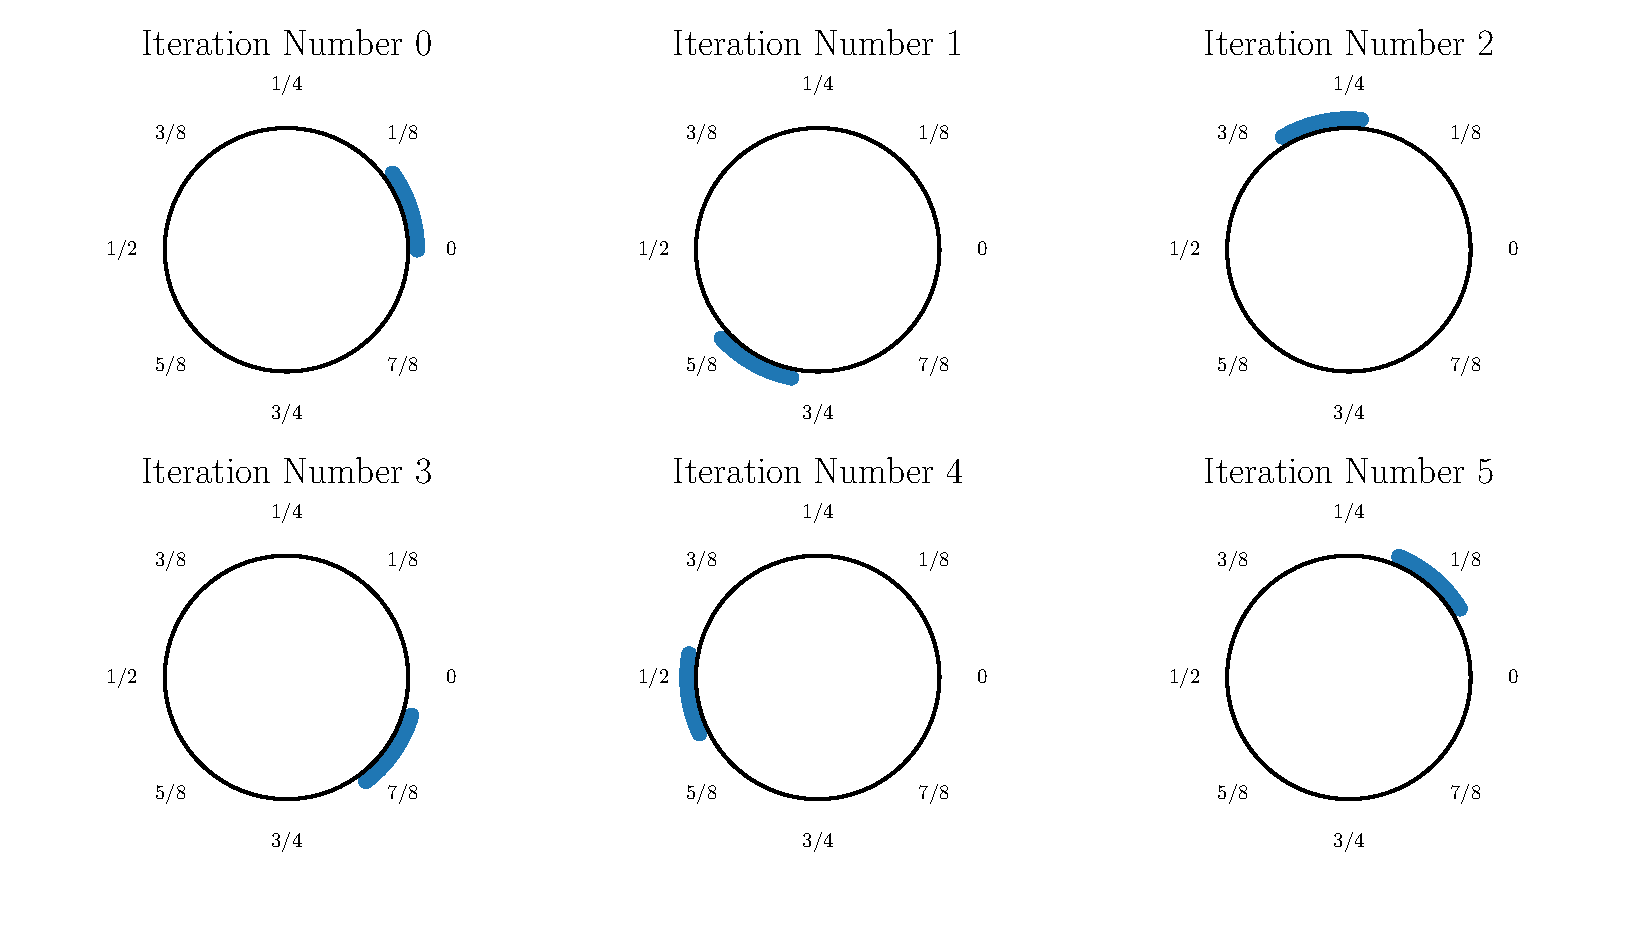
\includegraphics[scale = 0.6]{Q107_Ulam_Rot_34.eps}
	\caption{The first five rotations by a rational angle ($21/34$) of a mass distributed uniformly from 0 to 0.1.}
\end{figure}

\begin{figure}[H]
	\centering
	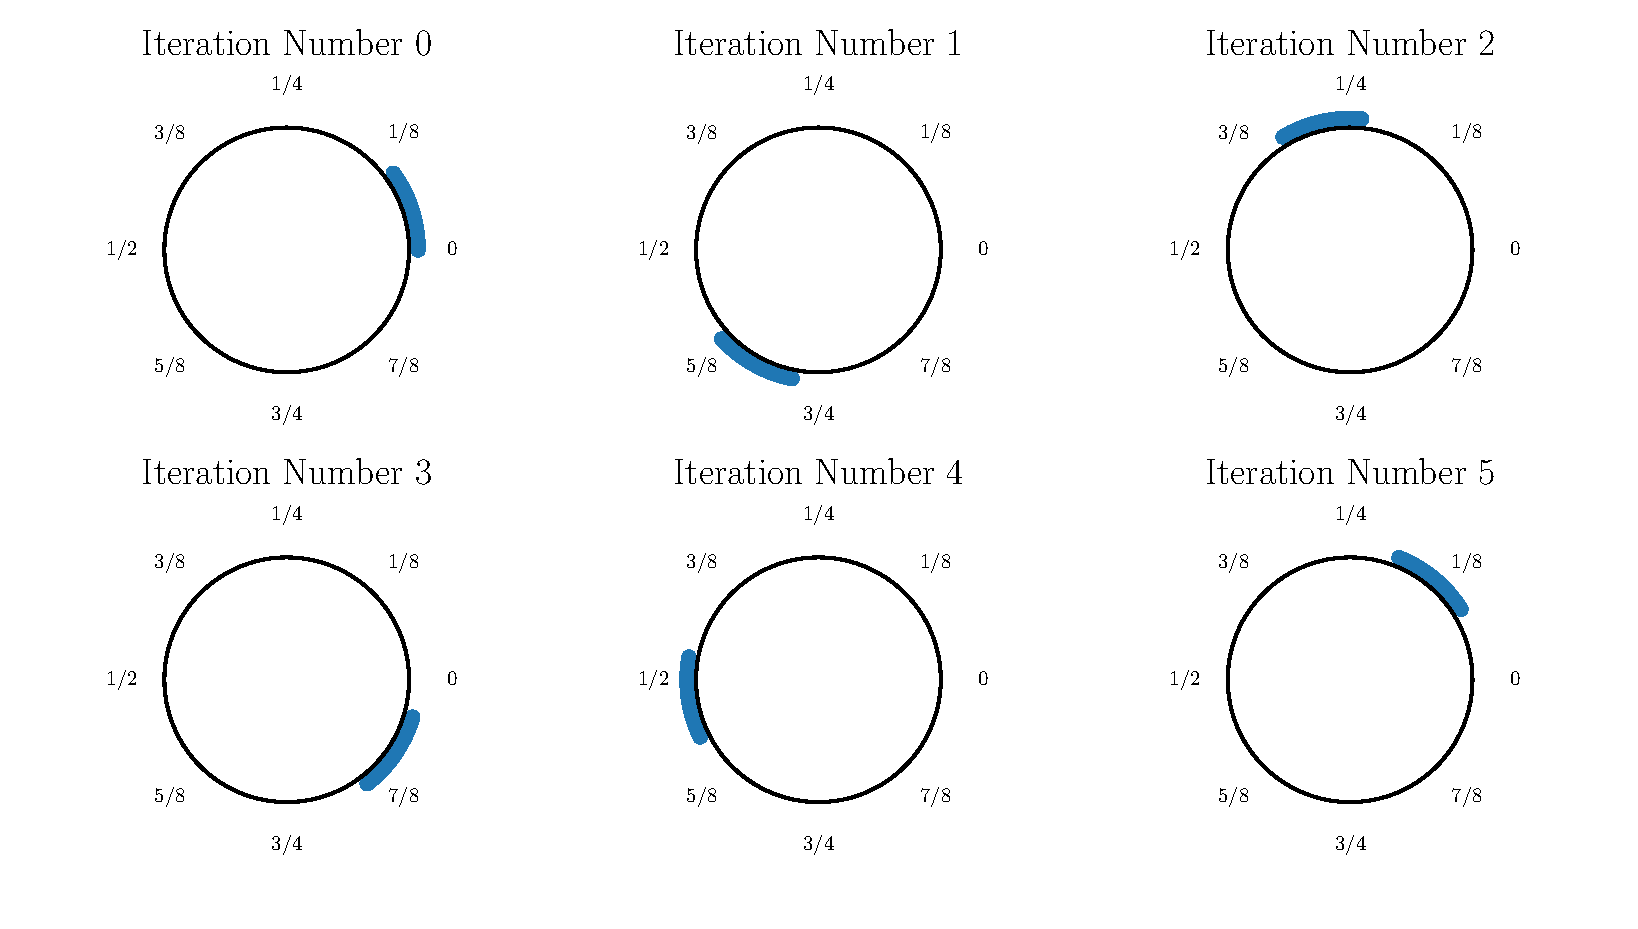
\includegraphics[scale = 0.6]{Q107_Ulam_Rot_root5.eps}
	\caption{The first five rotations by a irrational angle ($(\sqrt{5}-1)/2$) of a mass distributed uniformly from 0 to 0.1.}
\end{figure}

\end{appendices}

\end{document}
